\documentclass[a4paper,12pt]{scrreprt}
\usepackage[ngerman]{babel}
\usepackage[a4paper]{geometry}
\geometry{a4paper,total={170mm,257mm},left=20mm,top=15mm}
\usepackage{amsmath}
\usepackage{acronym}
\usepackage{graphicx}
\usepackage[onehalfspacing]{setspace}
\usepackage[colorlinks=true, allcolors=blue]{hyperref}
\newcommand{\dcplace}{Aachen}
\newcommand{\dcdate}{04. Mai 2025}
\newcommand{\dcauthorfirstname}{Max}
\newcommand{\dcauthorlastname}{Mustermann}


\begin{document}
\begin{titlepage}
	%ab hier kleinere Raender, mehr bedruckbare Flaeche.
	\thispagestyle{empty}
	\newgeometry{a4paper, portrait, left=1.0cm, right=0cm, top=0.6cm, bottom=0cm, includefoot}

    \noindent
    \begin{minipage}[t]{0.5\textwidth}
        
\includegraphics[width=3.7cm]{firmenlogo.jpg}
    \end{minipage}%
    \begin{minipage}[t]{0.5\textwidth}
          \raggedleft
          
\includegraphics[width=1.7cm]{FHAC.jpg}
    \end{minipage}

	\vspace{1.0cm}

	% Kopfzeile mit Fachbereich ...
	{\centering \bfseries \Large FH~Aachen \\
	\vspace{1cm}
	\normalsize Fachbereich\\
	Elektrotechnik und Informationstechnik \\
	Studiengang~Informatik \par}

	\vspace{1cm}
    
	{\centering \bfseries \large Bachelorarbeit \par}

	\vspace{1cm}

	\centering \begin{minipage}[t]{13cm}
		\centering \small Konzeption und prototypische Entwicklung einer webbasierten Applikation zur Wertschöpfung und Bereistellung von Geodaten \\
        (Data-Konnector für Geodaten)
		\medskip
	\end{minipage}

	\vspace{1.5cm}
    
	%\vspace*{1cm}
	%\hspace*{6.8cm}
	\begin{minipage}[t]{9cm}
		\centering Tuan Anh Cong Nguyen \\ Matr.-Nr.: 3517392
	\end{minipage}
	\vspace{2.1cm}
    
	%\vspace*{4.7cm}
	%\hspace*{6.8cm}
	\centering \begin{minipage}[b]{15cm}
		\centering
			Referent: Prof. Dr. rer. nat. Heinrich Faßbender\\
			%Korreferent: Prof. Dr.-Ing. ...\
	\end{minipage}


	\vspace{1.5cm}
	
	%Erstellungsdatum
	%\vspace{-4cm}
	%\begin{flushright}
	\centering %\hspace{8cm}
	\begin{minipage}[b]{10cm}
			\centering
            In Zusammenarbeit mit Ausbildungsbetrieb:\\
            ahu GmbH Wasser Boden Geomatik \\
            \vspace{1cm}
            Externer Betreuer: Dr. David Loibl
            
			%\today\\ %Datum\\
			%\vspace{1cm}
			%vertraulich bis xx.xx.xx
	\end{minipage}
	%\end{flushright}

	%\today
	\restoregeometry
\end{titlepage}

\clearpage % Neue Seite für Selbstständigkeitserklärung
\chapter*{Selbstständigkeitserklärung}
\thispagestyle{empty}	%keine Seitenzahl!
\pdfbookmark{Selbstständigkeitserklärung}{Selbstständigkeitserklärung}
Ich versichere hiermit, dass ich die vorliegende Arbeit selbständig verfasst und keine anderen als die im Literaturverzeichnis angegebenen Quellen benutzt habe.\\ \\
Stellen, die wörtlich oder sinngemäß aus veröffentlichten oder noch nicht veröffentlichten Quellen entnommen sind, sind als solche kenntlich gemacht.\\ \\ Die Zeichnungen oder Abbildungen in dieser Arbeit sind von mir selbst erstellt worden oder mit einem entsprechenden Quellennachweis versehen.\\ \\ Diese Arbeit ist in gleicher oder ähnlicher Form noch bei keiner anderen Prüfungsbehörde eingereicht worden.\\ \\[2ex]
Aachen, den \today \hspace{4cm} \dotfill 
\tableofcontents

\clearpage
\chapter*{Abkürzungsverzeichnis}\label{abkuerzungsverzeichnis}
\begin{acronym}[YTM]
\setlength{\itemsep}{-\parsep}

\acro{gravitation}[$g$]{\hspace{1cm}Gravitation in Nähe der Erdoberfläche}
\acro{Nu}[$Nu$]{\hspace{1cm}Nußelt-Zahl}
\acro{nu_luft}[$\nu_{Luft}$]{\hspace{1cm}Kinematische Viskosität von Luft}
\acro{Pr}[$Pr$]{\hspace{1cm}Prandtl-Zahl}
\acro{Q}[$\dot Q$]{\hspace{1cm}Wärmestrom}
\acro{Ra}[$Ra$]{\hspace{1cm}Rayleigh-Zahl}
\acro{rho_luft}[$\rho_{Luft}$]{\hspace{1cm}Dichte von Luft}
\acro{temperatur}[$T$]{\hspace{1cm}Temperatur}
\acro{umgebungstemperatur}[$T_{\infty}$]{\hspace{1cm}Umgebungstemperatur}

\end{acronym}

\cleardoublepage
\chapter*{Abstract}
\thispagestyle{plain}
\addcontentsline{toc}{chapter}{Abstract}
In einer zunehmend digitalisierten und automatisierten Welt wächst täglich die Menge an neu generierten Geodaten – insbesondere Mess- und räumlichen Daten.\\ \\
Die Suche nach und Einbindung von OGC-Geodatendiensten wie WMS (Web Map Service) und WFS (Web Feature Service) in Geoinformationssysteme wie QGIS kann tatsächlich schwierig sein. Die Suche erfordert den Anwender oft das Durchforsten verschiedener Quellen und die manuelle Überpüfung von Dienstbeschreibung. Eine automatisiert und effiziente Lösung kann teilweise helfen, diesen Prozess zu verbessern. \\ 
Die Suche nach Messdaten wie Grundwasserständen, Pegelständen und Klimadaten (Niederschlag,Temperatur) und deren Umformatierung in ein einheitliches Format gestalten sich als schwierig und kompliziert, da es eine Vielzahl von Datenanbietern mit unterschiedliche Datenstrukturen, Formen, etc. gibt.\\ \\
Die Bereitstellung dieser Rohdaten erfolgt meinst im CSV-Format oder als individuell strukturtierte ASCII-Dateien. Im Kontext von der Datenkonsum, gibt es bei der Ahu den sogenannten ahuManager-Client, der diese Daten konsumiert. Bevor diese konsumieren können, müssen die Rohdaten in ein kompatibeles Format umformatiert werden, was bisher teilweise von Hand erledigt werden (in Excel o.ä.). Diese manuelle Vorgehen kann perspektivisch zum Teil oder ganz automatisiert werden, was die Produktivität steigert und die Fehleranfälligkeit vermeidet. \\ \\
Daher befasst sich diese Arbeit  mit dem Thema, wie eine webbasierte Applikation zur Wertschöpfung und Bereitstellung von rohen Geodaten im Kontext von der Abteilung Geomatik von Ahu GmbH entwickelt werden kann.

\clearpage
\chapter{Einleitung}
\section{Motivation der Arbeit}
Diese Bachelorarbeit wird in Zusammenarbeit mit dem Bereich Geomatik der Ahu GmbH verfasst. Der Bereich beschäftigt sich mit Konzeption und Softwareentwicklung der Monitoringsysteme und Web-Anwedungen, die es Dienstleitern, Betreibern und Aufsichtsbehördern ermöglichen, ein kosteneffizientes Management für Geodaten (Grundwassser,Oberflächenwasser, Boden,etc.) umzusetzen. \\ \\
Momentan besteht es Bedarf für ein zentrales System zur automatisierten Suche und Verwaltung der Geodaten aus verschiedenen Datenanbietern und diese Daten in einer homogen Struktur zusammenzubringen und einen vorhandenen Client(z.B ahuManager) bereitzustellen. Unter anderem  wird auch die Einbindung von OGC-Geodatendiensten für besseren und effizienten Prozess zur Durchsuche und Verwaltung gesorgt. 

\section{Ziel der Arbeit}
Die Hauptaufgabe dieser Arbeit besteht darin, ein Konzeption für die prototypische Entwicklung einer webbasierten Applikation zu erstellen und umzusetzen. Die Ziele der Applikation enthalten eine übergreifende Suche von Geodaten und deren Umformatierung in ein passendes vorgegebenes Zielformat. Das weitere Zeil ist die Einbindung von mindenstens einer OGC-Geodatendiensten.\\ \\ Durch die Umsetzungen dieser Ziele soll perspektivisch eine Software entstehen, die die offenen Problematik abdeckt.

\chapter{Some examples to get started}
\section{How to create Sections and Subsections}

\section{How to include Figures}
Note that your figure will automatically be placed in the most appropriate place for it, given the surrounding text and taking into account other figures or tables that may be close by. You can find out more about adding images to your documents in this help article on \href{https://www.overleaf.com/learn/how-to/Including_images_on_Overleaf}{including images on Overleaf}.
\subsection{How to add Tables}

\begin{figure}
\centering
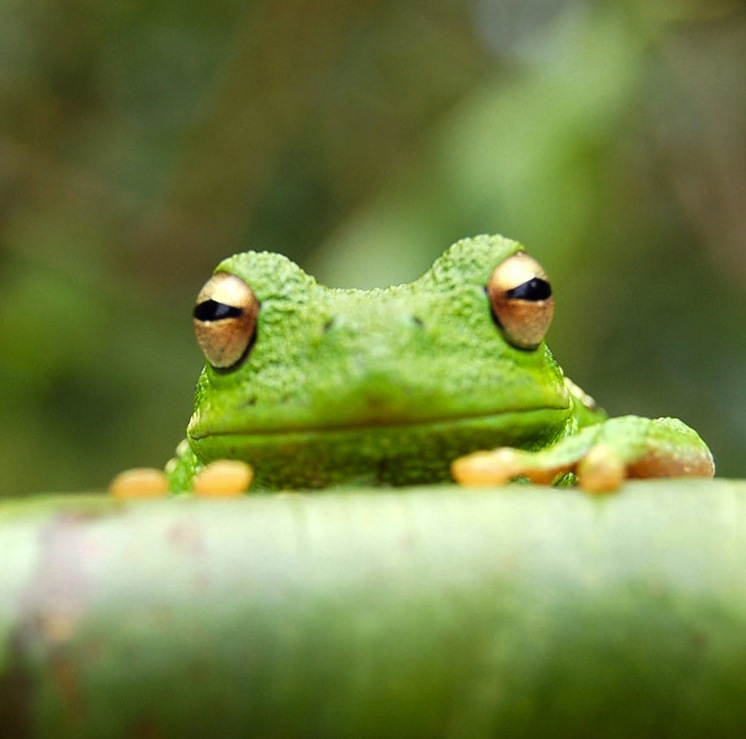
\includegraphics[width=0.25\linewidth]{frog.jpg}
\caption{\label{fig:frog}This frog was uploaded via the file-tree menu.}
\end{figure}


Use the table and tabular environments for basic tables --- see Table~\ref{tab:widgets}, for example. For more information, please see this help article on \href{https://www.overleaf.com/learn/latex/tables}{tables}. 

\begin{table}
\centering
\begin{tabular}{l|r}
Item & Quantity \\\hline
Widgets & 42 \\
Gadgets & 13
\end{tabular}
\caption{\label{tab:widgets}An example table.}
\end{table}

\section{How to add Comments and Track Changes}

Track changes are available on all our \href{https://www.overleaf.com/user/subscription/plans}{premium plans}, and can be toggled on or off using the option at the top of the Review pane. Track changes allow you to keep track of every change made to the document, along with the person making the change. 

\section{How to add Lists}

You can make lists with automatic numbering \dots

\begin{enumerate}
\item Like this,
\item and like this.
\end{enumerate}
\dots or bullet points \dots
\begin{itemize}
\item Like this,
\item and like this.
\end{itemize}

\section{How to write Mathematics}

\LaTeX{} is great at typesetting mathematics. Let $X_1, X_2, \ldots, X_n$ be a sequence of independent and identically distributed random variables with $\text{E}[X_i] = \mu$ and $\text{Var}[X_i] = \sigma^2 < \infty$, and let
\[S_n = \frac{X_1 + X_2 + \cdots + X_n}{n}
      = \frac{1}{n}\sum_{i}^{n} X_i\]
denote their mean. Then as $n$ approaches infinity, the random variables $\sqrt{n}(S_n - \mu)$ converge in distribution to a normal $\mathcal{N}(0, \sigma^2)$.

\section{How to change the margins and paper size}
If however you're using a more general template, such as this one, and would like to alter the margins, a common way to do so is via the geometry package. You can find the geometry package loaded in the preamble at the top of this example file, and if you'd like to learn more about how to adjust the settings, please visit this help article on \href{https://www.overleaf.com/learn/latex/page_size_and_margins}{page size and margins}.

\section{How to change the document language and spell check settings}
\href{https://www.overleaf.com/learn/latex/International_language_support}{international language support}.

\section{How to add Citations and a References List}
You can simply upload a \verb|.bib| file containing your BibTeX entries, created with a tool such as JabRef. You can then cite entries from it, like this: \cite{greenwade93}. Just remember to specify a bibliography style, as well as the filename of the \verb|.bib|. You can find a \href{https://www.overleaf.com/help/97-how-to-include-a-bibliography-using-bibtex}{video tutorial here} to learn more about BibTeX.
If you have an \href{https://www.overleaf.com/user/subscription/plans}{upgraded account}, you can also import your Mendeley or Zotero library directly as a \verb|.bib| file, via the upload menu in the file-tree.

\section{Good luck!}
We hope you find Overleaf useful, and do take a look at our \href{https://www.overleaf.com/learn}{help library} for more tutorials and user guides! Please also let us know if you have any feedback using the Contact Us link at the bottom of the Overleaf menu --- or use the contact form at \url{https://www.overleaf.com/contact}.

\chapter{Übersicht von Technologien}
\section{Vaadin}
Vaadin ist ein serverseitiges Web-Framework, das dem Entwickler erlaubt, moderne Webanwendung in Java zu entwicklen, ohne dass explizit HTML,CSS oder JavaScript geschrieben werden muss. Vaddin verfügt über eine große Komponentenbibliothek, die eine Vielzahl an vorgefertigten UI-Elementen wie Buttons, Tabellen, Formulare, Dialoge und Layouts bietet. \\ \\
Vaadin verfolgt einen serverseitigen Rendering-Ansatz. Während eine AJAX-basierte Vaadin Client-Side Engine dafür sorgt, dass die Benutzeroberfläche im Browser durch ein Widget-Set gerendert wird. Die Benutzeroberfläche kann aus eingebauten Komponenten, Add-Ons und benutzerdefinierten Komponenten bestehen. Diese Client-Side Engine kommuniziert über HTTP oder WebSockets mit dem Server. Die gesamte UI-Logik wird dann auf dem Server ausgeführt. Die Vaadin Servlet empfängt Client-Anfragen und aktualisiert die Benutzeroberfläche. Die UI-Komponenten werden serverseitig erstellt und verwaltet. Änderungen in der UI werden durch die Vaddin Client-Side Engine an den Browser zurückgespielt.  
\begin{figure}[h!]
\centering
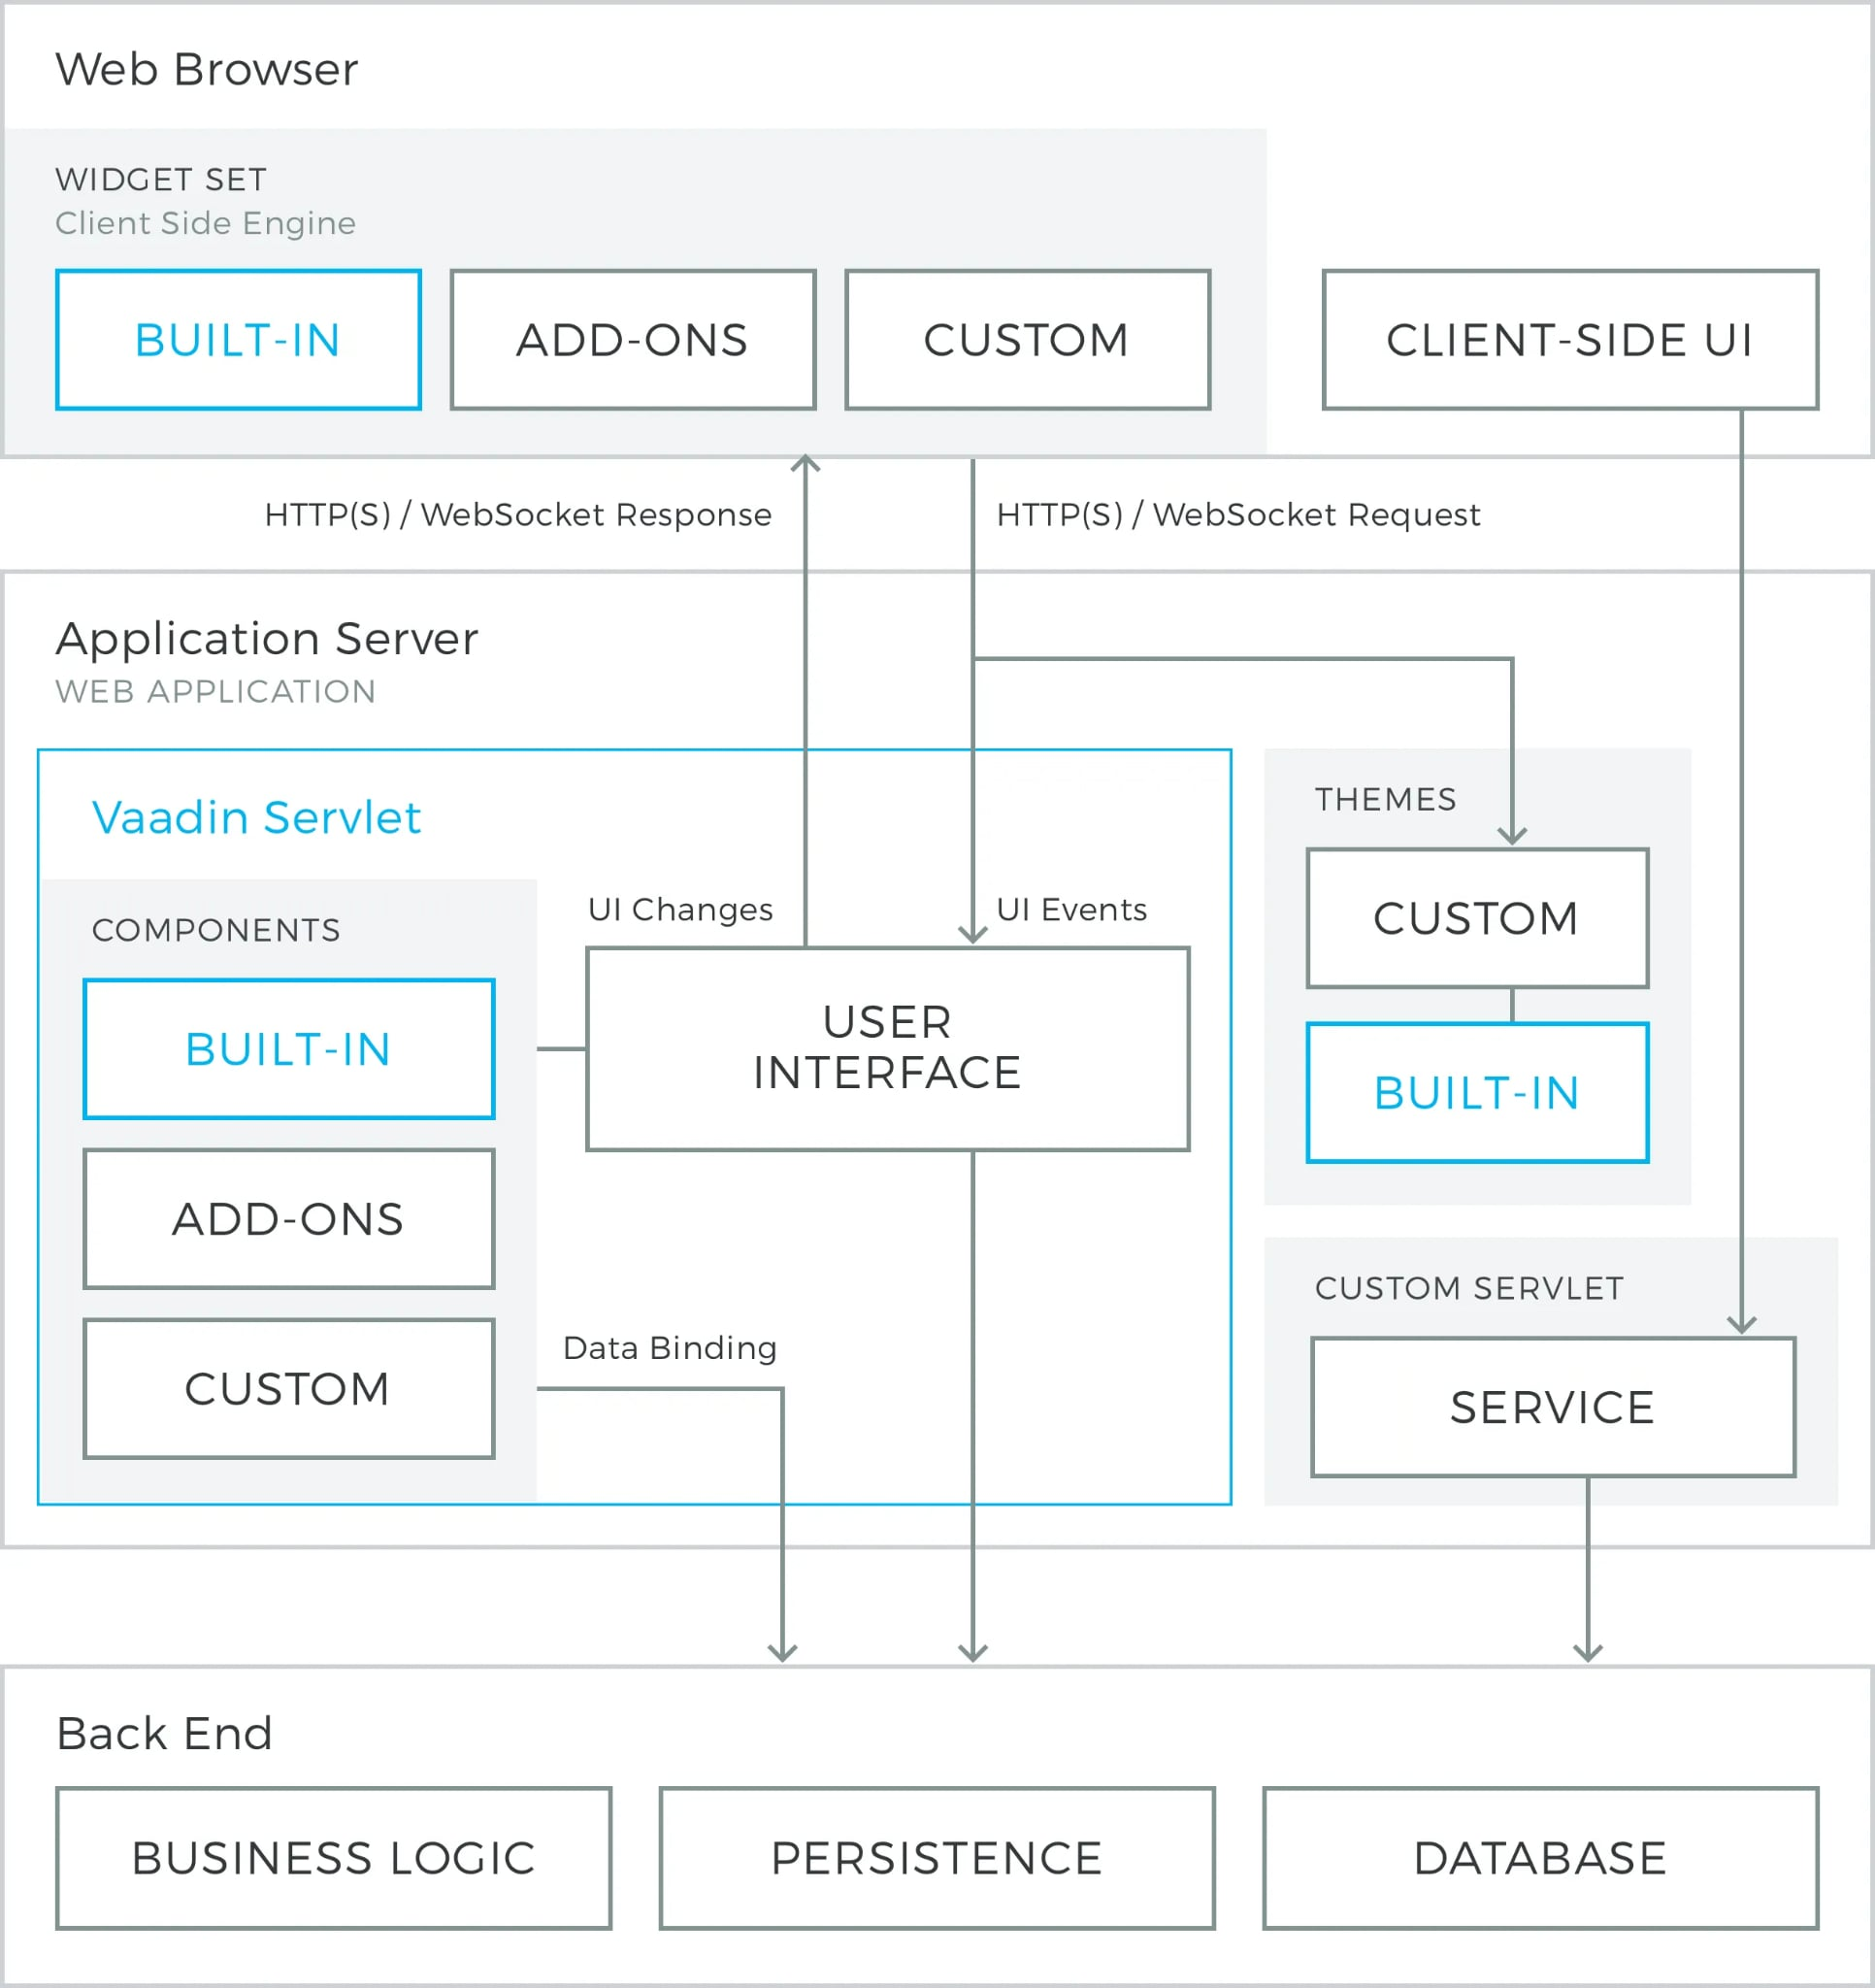
\includegraphics[width=9cm, height=10cm]{vaadin_architekture.jpg}
\caption{\label{vaadin:architektur}Übersicht \href{https://vaadin.com/docs/v8/framework/architecture/architecture-overview} {Vaadin Architektur}}
\end{figure}

\section{Spring Framework}
Spring Framework ist ein Java-Framework, das um 2003 als Reaktion auf die damals noch zu komplizierte J2EE-Platform entwickelt wurde. Spring ermöglicht eine einfachere und unkompliziertere Entwicklung von Enterprise-Applikation in Java. Eines der wichtigsten Konzepte von Spring war die Inversion of Control (IoC).
IoC ist ein Prinzip, bei dem der Kontrollfluss an eine externe Quelle(z.B. ein Framework) übergeben wird. Das Framework ist dann gemäß einer Spezifikation für die Erstellung und Löschung der Objekte und den Aufruf von Methoden verantwortlich. \\ \\ Spring führt das Konzept des Bean-Containers ein. Beans sind Java-Objekte, die von Spring instanziiert und verwaltet sind. Wenn die Haupt-Bean von der Hilfs-Bean abhängig ist, stellt Spring sicher, dass die Hilfs-Bean vor der Haupt-Bean initialisiert wird. Spring injizierte außerdem die Instanz der Hilfs-Bean in die Haupt-Bean, sodass die Haupt-Bean nicht mehr nach ihren eigennen Abhängigkeiten suchen muss. Dieses Muster wird als Dependendy Injection bezeichnet.\\ \\
Damals musste der Entwickler die Bean-Konfiguration in XML schreiben, die Spring anweist, wie die Beans zu konsutruieren sind. Inzwischen wird diese mithilfe einer Kombination aus Java-Annotation, Java-Code und Konventionen erstellt.
\section{Spring Boot}
Mit dem Wachstum der Spring-Plattform nahm auch die Komplexität der Entwicklung von Spring-Anwendungen zu. Gleichzeitig verbreitet sich der Einsatz von Microservices und containerisierten Umgebungen in der SOftwareentwicklung. Entwickler wünschten sich einfach Methode, um schlanke Webanwendungen zu erstellen, die unabhängig als eigenständige Dienst ausgeführt werden können, anstatt auf einem dedizierten Anwendungsserver zu laufen.\\ \\
Spring Boot wurde als Reaktion auf diese Anforderungen entwickelt. Es erleichtert die Erstellung von Spring-Anwendungen durch sinnvolle Standard-Einstellungen, Starter-Abhängigkeiten und produktionsreife Funktionen für Konfiguration und Überwachung. Durch die Einführung eingebetteter Servlet-Container wurde es möglich, Anwendungen als eigenständige, ausführbare JAR-Dateien zu verpacken. 
\section{Maven}
Maven ist ein Build-Management- und Projektverwaltungswerkzeug, das häufig in der Java-Entwicklung eingesetzt wird. Es automatisiert Aufgaben wie das Herunterladen von Abhängigkeiten, das Kompilieren von Quellcode und das Ausführen von Builds sowie Tests. Maven verwendet eine zentrale Konfigurationsdatei, die \texttt{pom.xml}, um alle Aspekte des Projekts wie Libraries, Plugins und Build-Prozesse zu steuern.\\ \\
Die Funktionsweise von Maven baisert auf einem deklaravitven Ansatz. Das bedeutet, dass der Entwickler alle relevanten Informationen über das Projekt in einer zentralen Konfigurartionsdatei, der sogenannten \texttt{pom.xml}( Projekt Object Model) angibt, wie z.B. Abhängigkeiten, Build-Prozesse und Plugins.
\section*{\small \textbf{1. Die pom.xml-Datei (Project Object Model)}}
Die \texttt{pom.xml} ist das Herzstück eines Maven-Projekts. Sie enthält Informationen wie:
\begin{itemize}
\item Projektinformationen: Name des Projekts, Version, Beschreibung.
\item Anhängigkeiten: Welche Bibliotheken und Framworks das Projekt benötigt.
\item Plugins: Zusätzliche Werkzeuge, die den Build-Prozess erweitern (z.B. Compiler-Plugins, Test-Frameworks).
\item Repositories: Woher Maven externe Abhängigkeiten herunterladen soll, typischerweise das Maven Central Repository.
\item Build-Spezifikationen: Kompilierungsanweisungen, Testkonfigurationen und Deployment-Optionen.
\end{itemize}
\section*{\small \textbf{2. Build-Lifecycle}}
Maven besitzt einen vordefinierten Build-Lifecycle, der aus mehreren Phasen besteht. Zu den wichtigsten Phasen gehören:
\begin{itemize}
\item validate: Überprüft, ob alle erforderlichen Informationen im Projekt vorhanden sind.
\item compile: Kompiliert den Quellcode.
\item Führt automatisierte Tests aus.
\item package: Verpackt den kompilierten Code in ein Distributionsformat, typischerweise eine JAR- oder WAR-Datei.
\item install: Installiert das Paket in das lokale Maven-Repository, damit es in anderen Projekten verwendet werden kann.
\end{itemize}

\bibliographystyle{alpha}
\bibliography{sample}
\end{document}